%\documentclass[multi,preview,varwidth=false,border=5,12pt]{standalone}
\documentclass[12pt]{article}

\newcounter{Qnum}
\usepackage{assignments}
%\standaloneenv{question}


%\excludecomment{solution}\let\endsolution\relax


\begin{document}


\begin{center}
\section*{Nature of fluids}
\end{center}

\begin{question}
A test mass used by the LISA Pathfinder mission is a cube of solid gold--platinum alloy, measuring 4.6 cm on a side and weighing 1.96 kg.  Compute the cube's density, specific weight and specific gravity.

\begin{solution}
  We start by computing the cube's density which is its mass divided by its volume.  Since we want our answer to be in units of $\kg/\m^3$ we first convert the length of the side from 4.6 cm to 0.046 m.  The volume is therefore $V=\left(0.046~\m\right)^3=9.73\times 10^{-5}~\m^3$.
  \begin{align*}
  \rho=\frac{m}{V}=\frac{1.96~\kg}{9.73\times 10^{-5}~\m^3}=20,144~\kg/\m^3
  \end{align*}
  This is a reasonable result as it falls between the densities of platinum and gold which are $21,450~\kg/\m^3$ and  $19,300~\kg/\m^3$ respectively. [https://physics.info/density/]

  The specific weight is then computed from
  \begin{align*}
  \gamma=\rho g=20,144~\kg/\m^3\times 9.81~\m/s^2=1.976\times 10^5~\N/\m^3
  \end{align*}

  Finally, the specific gravity can be computed as
  \begin{align*}
  sg=\frac{1.976\times 10^5~\N/\m^3}{9.81\times 10^3~\N/\m^3}=20.144
  \end{align*}
\end{solution}
\end{question}


\begin{question}
Air at $40\C$ and standard atmospheric pressure has a specific weight of 11.05 N/m$^3$.
Calculate its density.

\begin{solution}
  We can use the relation $\gamma=\rho g$ to find the density from the specific weight.
  \begin{align*}
      \rho=\frac{\gamma}{g}=\frac{11.05~\N/\m^3}{9.81~\m/s^2}=1.126~\kg/\m^3
  \end{align*}
\end{solution}

\end{question}


\begin{question}
A storage vessel for gasoline (sg=0.68) is a vertical cylinder 10 m in diameter.  If it is filled to a depth of 6.75 m, calculate the weight and mass of the gasoline.

\begin{solution}
  This is a two step problem.  First we will use the specific gravity to compute the density and specific weight.

  \begin{align*}
    \rho_{\rm gas}&=sg\times \rho_{\rm water}=0.68\times 1000~\kg/\m^3=680~\kg/\m^3\\
    \gamma_{\rm gas}&=sg\times \gamma_{\rm water}=0.68\times 9.81~\kN/\m^3=6.67~\kN/\m^3
  \end{align*}

  Then using the volume of gasoline we will get the total weight and mass.  The volume of gasoline is the volume of the cylinder as described.

  \begin{align*}
      V={\rm Height}\times {\rm Area}=6.75~\m\times \left(\frac{\pi (10~\m)^2}{4}\right)=530~\m^3
  \end{align*}

  The mass and weight is therefore

  \begin{align*}
      m&=\rho\times V=680~\frac{\kg}{\m^3}\times 530~\m^3 = 3.6\times 10^{5}~\kg\\
      w&=\gamma\times V=6.67~\frac{\kN}{\m^3}\times 530~\m^3 = 3500~\kN
  \end{align*}

\end{solution}

\end{question}

\begin{question}
A storage vessel for gasoline (sg=0.68) is a vertical cylinder 30~ft in diameter.  If it is filled to a depth of 22~ft, calculate the number of gallons and weight of the gasoline.

\begin{solution}
  This question is similar to the one before except now that it asks for the weight of the gasoline (in pounds) and the volume (in gallons).  The specific weight of the gasoline is

  \begin{align*}
    \gamma_{\rm gas}=sg\times \gamma_{\rm water}=0.68\times 62.4~\lb/\ft^3=42.4~\lb/\ft^3
  \end{align*}

  Then using the volume of gasoline we will get the total weight.  The volume of gasoline is the volume of the cylinder as described.

  \begin{align*}
      V={\rm Height}\times {\rm Area}=22~\ft\times \left(\frac{\pi (30~\ft)^2}{4}\right)=15550~\ft^3
  \end{align*}

  The weight is therefore

  \begin{align*}
      w=\gamma\times V=42.4~\frac{\lb}{\ft^3}\times 15550~\ft^3 = 6.60\times 10^5~\lb
  \end{align*}

  The volume in gallons is

    \begin{align*}
      V==15550~\cancel{\ft^3}\times\left(\frac{7.48~\gal}{\cancel{\ft^3}}\right)=1.16\times 10^5~\gal
  \end{align*}

\end{solution}

\end{question}


\begin{question}
Liquid ammonia has a specific gravity of 0.826.  Calculate the volume in cm$^3$  that would weigh 5.0 lb.

\begin{solution}
 2745~cm$^3$
\end{solution}

\end{question}

\begin{question}
What is the specific gravity of 38$^\circ$ API oil?

\end{question}

\begin{question}
A hydraulic press that must exert a force of 4000~lbs operates with a 2~in diameter cylinder.  Compute the required oil pressure.

\begin{solution}
1273~psi
\end{solution}


\end{question}

\begin{question}
The maximum pressure a fluid power cylinder can sustain is 25.0 MPa.  Compute the minimum diameter necessary for the piston to exert a force of 50~kN.

\begin{solution}
50.5~mm
\end{solution}

\end{question}

\begin{question}
A hydraulic system operates using machine oil having a bulk modulus $K=189,000~\psi$.  What is the percentage change in volume as the system pressure is increased from zero to 4000 psi?

\begin{solution}
-2.1 percent
\end{solution}

\end{question}

\begin{question}
A hydraulic cylinder filled with water has an inside diameter of 1.0~in and a length of 2.0~ft. How many pounds of force must be applied to a piston at the end of the cylinder to compress the water by 0.25~in?

\begin{solution}
2585~lbs
\end{solution}

\end{question}

\begin{question}

Which of the following phenomena is {\bf not} related to the consideration of vapor pressure.

\begin{enumerate}
  \item brake fade
  \item cavitation
  \item shear thinning
  \item vapor lock
\end{enumerate}

\begin{solution}
shear thinning
\end{solution}

\end{question}

\begin{question}

Which fluid property allows insects like the water strider and arachnids like the fisher spider to walk on water?

\begin{enumerate}
  \item viscosity index
  \item surface tension
  \item compressibility
  \item vapor pressure
\end{enumerate}

\begin{solution}
surface tension
\end{solution}

\end{question}


\begin{question}
Convert a dynamic viscosity measurement of 2500~cP into $\Pa\cdot \s$.

\begin{solution}
$2.5~\Pa\cdot \s$
\end{solution}
\end{question}


\begin{question}

 Estimate the shear viscosity (in centipoise) of castor oil using the experimental viscometer data shown in the figure below.

 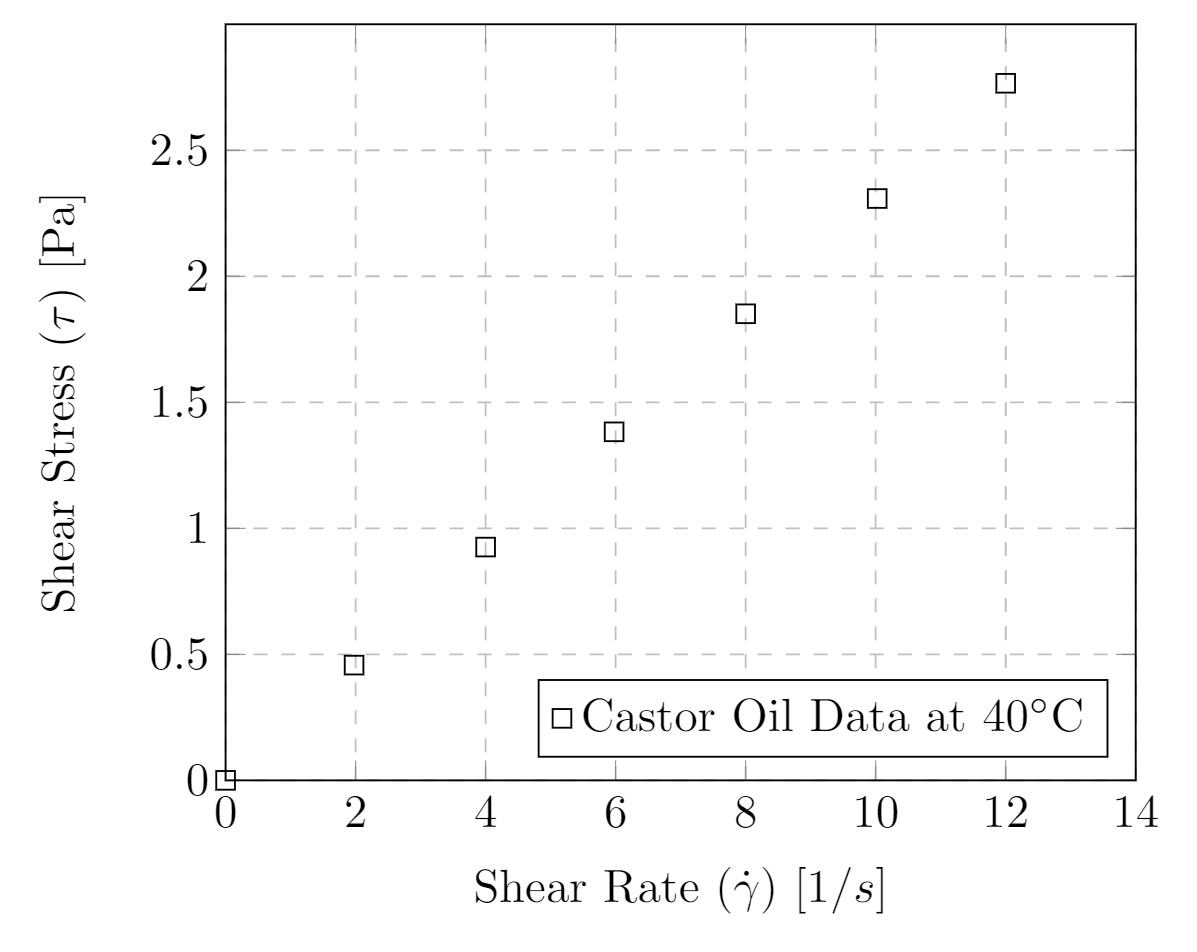
\includegraphics[width=4in]{imgs/CastorOil.png}

\begin{solution}
231 cP
\end{solution}
\end{question}

\begin{question}

The following three questions are based on the experimental viscometer data for French dressing shown in the figure below.

 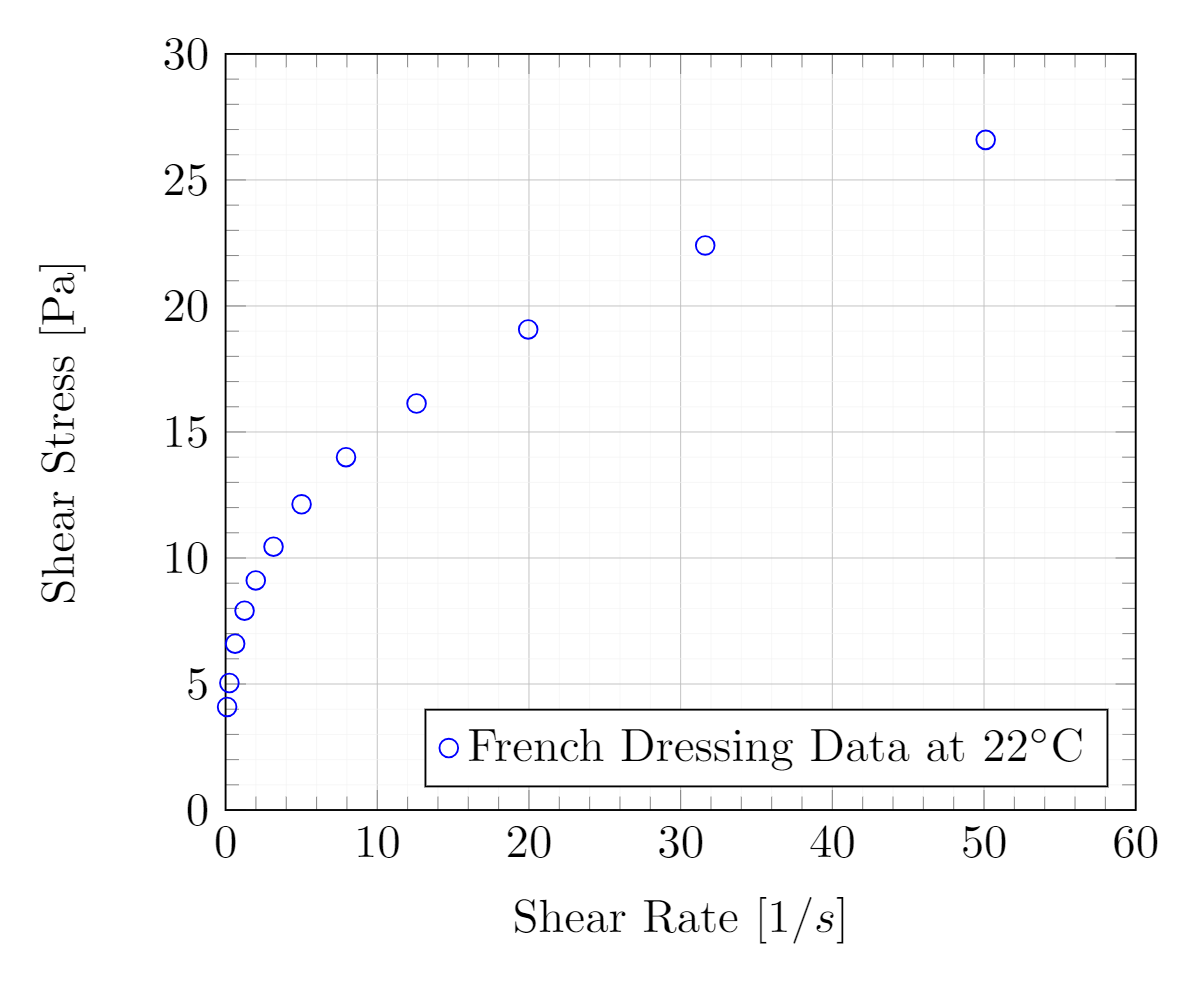
\includegraphics[width=4in]{imgs/FrenchDressing.png}

What best describes the viscous behavior of French dressing?

\begin{enumerate}
  \item Bingham
  \item Dilatant (shear thickening)
  \item Newtonian
  \item Pseudoplastic (shear thinning)
\end{enumerate}

\begin{solution}
Pseudoplastic (shear thinning)
\end{solution}

\end{question}


\begin{question}

 Estimate the apparent viscosity of French dressing (in centipoise) at a shear rate of $\dot{\gamma}=10 s^{-1}$.

\begin{solution}
458 cP
\end{solution}

\end{question}

\begin{question}

 Estimate the apparent viscosity of French dressing (in centipoise) at a shear rate of $\dot{\gamma}=40 s^{-1}$.

\begin{solution}
227 cP
\end{solution}

\end{question}


\begin{question}

Does the viscosity of most liquids increase or decrease with temperature?

\begin{solution}
decrease
\end{solution}

\end{question}

\begin{question}

Does the viscosity of most gases increase or decrease with temperature?

\begin{solution}
increase
\end{solution}

\end{question}

\begin{question}

Two oils have the same kinematic viscosity at room temperature.  Oil brand A has a viscosity index ($VI$) of 100.  Oil brand B has a VI of 220.  At a temperature of $-10^\circ {\rm C}$ which oil brand has a lower viscosity.

\begin{solution}
Oil brand B
\end{solution}

\end{question}

\begin{question}

If you were asked to check the viscosity of an oil described as SAE 15W, at what temperatures would you make the measurements?

\begin{solution}
 $-20^\circ {\rm C}, -25^\circ {\rm C}, 100^\circ {\rm C}$
\end{solution}

\end{question}

\begin{question}

If you were asked to check the viscosity of an oil described as SAE 50, at what temperatures would you make the measurements?

\begin{solution}
$100^\circ {\rm C},  150^\circ {\rm C}$
\end{solution}

\end{question}

\begin{question}

Which of the following statements are true for two oils described as SAE 40 and SAE 110.

\begin{enumerate}
  \item The SAE 110 oil has a higher viscosity
  \item The SAE 40 oil has a higher viscosity
  \item The SAE 40 oil is for engine crankcase lubrication and the SAE 110 is for lubricating automotive gear transmissions
  \item The SAE 110 oil is for engine crankcase lubrication and the SAE 40 is for lubricating automotive gear transmissions
\end{enumerate}

\begin{solution}
The SAE 40 oil is for engine crankcase lubrication and the SAE 110 is for lubricating automotive gear transmissions
\end{solution}

\end{question}

\begin{question}

What is the maximum kinematic viscosity at $40^\circ {\rm C}$ of an oil described as ISO VG 460?  Express your answer in cSt.  $1~{\rm cSt}=1~{\rm mm}^2/s$.

\begin{solution}
506~cSt
\end{solution}

\end{question}


\end{document}
